\section{Анализ и проектирование системы компьютерного зрения в антропометрии}
Жизненный цикл программы в целом не может быть разделен на периоды. Он описывает процесс создания, тестирования и поддержания работы системы \ref{img33}.

\begin{figure}[ht!]
\centering
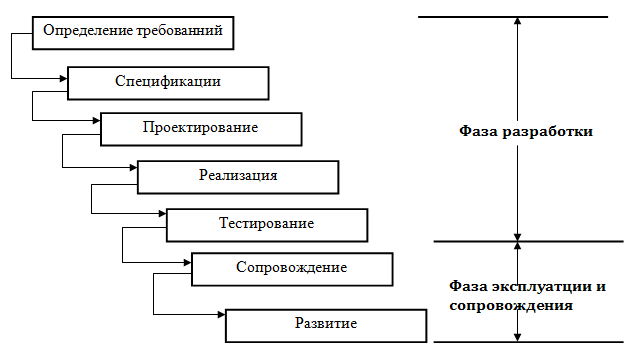
\includegraphics [scale=1] {images/h33.png}
\begin{center}
%\captionsetup{justification=justified, labelsep=period}
\caption{Общепринятая модель жизненного цикла программного обеспечения.} \label{img33}
\end{center}
\end{figure}

В данной работе подробно описан этап проектирования системы. Для этого было создано хранилище документов проекта, включающее в себя: теории и модели, методы и инструменты, используемые для создания и развития системы. Анализ и проектирование системы основаны на двух факторах: 

\begin{itemize}
	\item Понимание целей, структуры и процессов работы системы;
  \item Применение передовых методов и соответствующих алгоритмов для повышения эффективности работы и точности системы.

\end{itemize}
Особенностью анализа и объектно-ориентированного проектирования является система, включающая в себя совокупность объектов, взаимодействующих друг с другом для выполнения задачи с  достижением более высоких результатов. Для достижения этой цели мы должны использовать системные модели объектов со следующими основными характеристиками:

\begin{itemize}
	\item С высокой абстракцией;
  \item По состоянию упаковочной информации;
  \item Модуль;
  \item Наследование.

\end{itemize}
Сегодня UML является инструментом, обладающим  всеми характеристиками и условиями,о которых говорилось выше, для построения модели объекта. UML - графический язык для документирования, конструирования, описания параметров и визуализации абсолютно различных систем (программ в частности).
Графики моделирования объектов представлены в диссертации, в том числе:

\begin{itemize}
	\item \textbf{Диаграмма прецедентов} (Use Case diagram) - диаграмма, отражающая отношения между актёрами и прецедентами, являющаяся составной частью модели прецедентов, позволяющей описать систему на концептуальном уровне;
\item \textbf{Диаграмма классов} (Static Structure diagram) - диаграмма, демонстрирующая классы системы, их атрибуты, методы и взаимосвязи между ними. Входит в UML;
\item \textbf{Диаграмма последовательности} (sequence diagram): диаграмма, на которой для некоторого набора объектов на единой временной оси показан жизненный цикл (создание-деятельность-уничтожение) и взаимодействие (отправка запросов и получение ответов). Используется в языке UML.

\end{itemize}

Объектная модель описывает структуру объектов, их операции, атрибуты  и взаимосвязи с другими объектами. Объектная модель показывает понятия и реальные объекты, которые важны для разрабатываемой системы. Цель разработки объектной модели - выделение и описание объектов, составляющих проектируемую систему и выявление различных зависимостей между объектами.

Система компьютерного зрения в антропометрии включает в себя следующие основные вопросы:

\begin{itemize}
	\item Сбор и обработка данных с камеры;
	\item Извлечение антропометрических признаков;
	\item Классификация антропометрических данных;
	\item Разработка приложений для текстильной промышленности (E-Tailor) и фитнеса (E-фитнес) на основе результатов системы компьютерного зрения в антропометрии.
\end{itemize}

\begin{figure}[ht!]
\centering
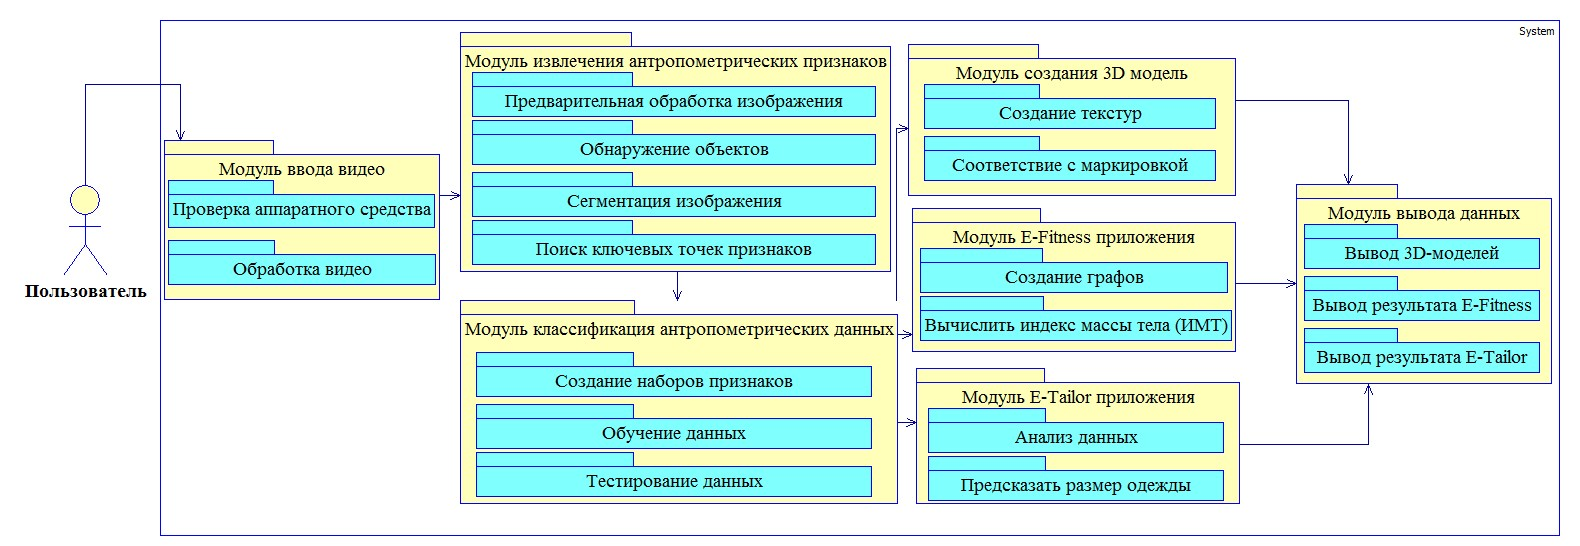
\includegraphics [scale=0.4] {images/h35.png}
\begin{center}
\caption{Структура ПО} \label{img35}
\end{center}
\end{figure}

\subsection{Анализ и проектирование системы компьютерного зрения в антропометрии для текстильной промышленности}

\textbf{Цель}: Описание работы программы автоматического измерения размеров человеческого тела, 3D моделирование тела мужчины / женщины, выбор размеров одежды на основе антропометрических признаков.

Система состоит из одного главного фактора: пользователи. Система имеет основные функции:

\begin{itemize}
	\item Сбор данных с камеры;
	\item Заполнение информации о росте, весе;
	\item 3D-моделирование человеческого тела;
	\item Классификация и предсказание размеров одежды;
	\item Контакты с командой разработчиков.

\end{itemize}
\begin{figure}[ht!]
\centering
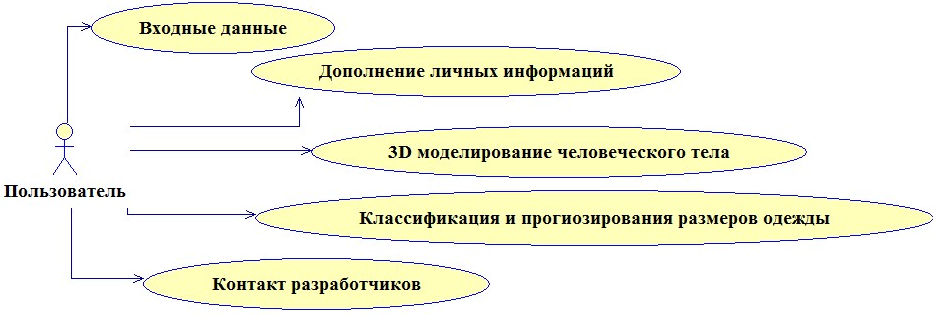
\includegraphics [scale=0.5] {images/h22.png}
\begin{center}
%\captionsetup{justification=justified, labelsep=period}
\caption{Диаграмма прецедентов - использование системы компьютерного зрения приложения E-Tailor.} \label{img22}
\end{center}
\end{figure}
\begin{figure}[ht!]
\centering
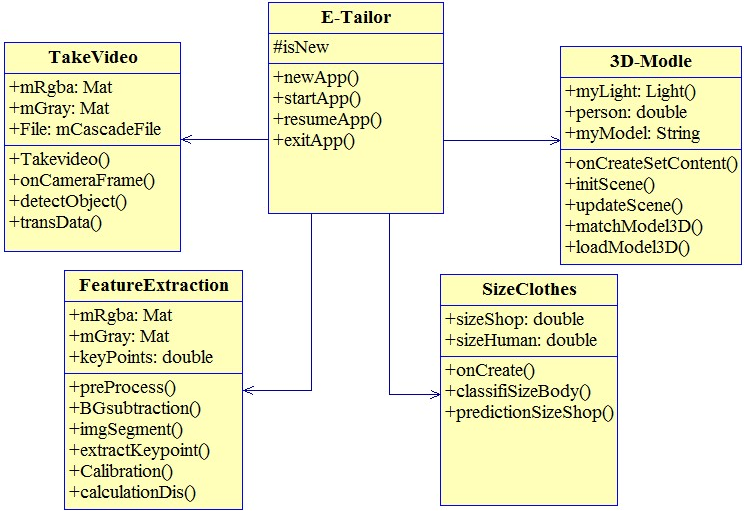
\includegraphics [scale=0.5] {images/h23.png}
\begin{center}
%\captionsetup{justification=justified, labelsep=period}
\caption{Диаграмма классов - система компьютерного зрения в антропометрии приложения E-Tailor.} \label{img23}
\end{center}
\end{figure}
\begin{figure}[ht!]
\centering
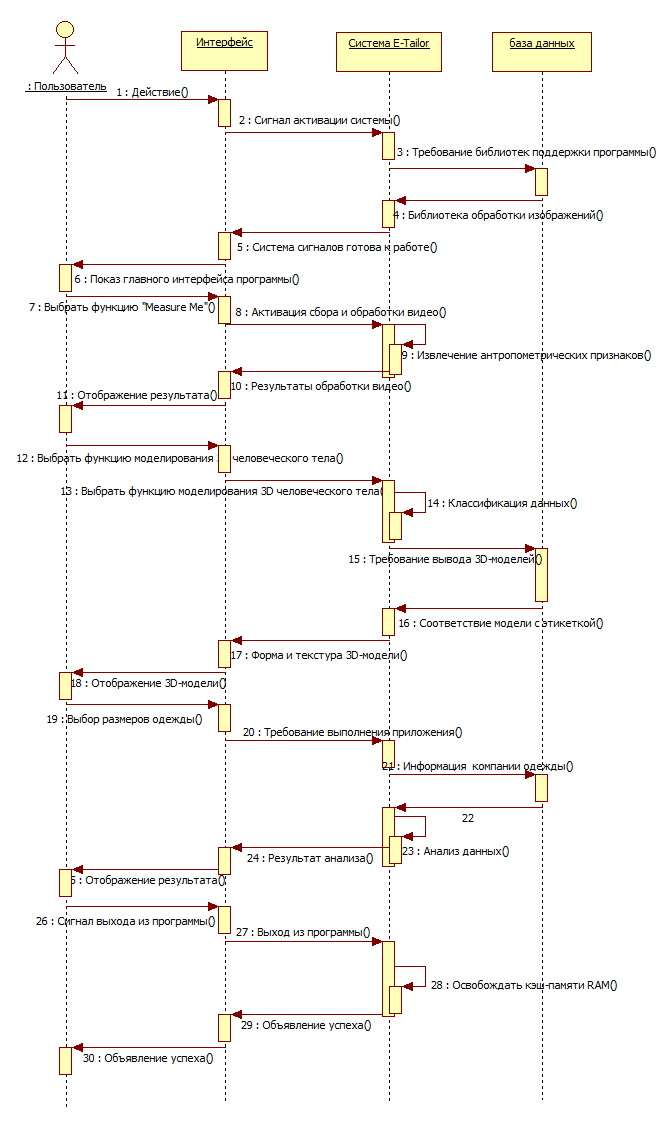
\includegraphics [scale=0.8] {images/h28.png}
\begin{center}
%\captionsetup{justification=justified, labelsep=period}
\caption{Диаграмма последовательности - система компьютерного зрения в антропометрии приложения E- Tailor.} \label{img28}
\end{center}
\end{figure}

\subsection{Анализ и проектирование системы компьютерного зрения в антропометрии для фитнеса}
\textbf{Цель}: Описание работы программы автоматического измерения размеров человеческого тела, 3D моделирование тела мужчины / женщины, автоматизация измерения индекса массы тела (ИМТ), анализ антропометрических признаков по стандартам фитнеса.

Система состоит из одного главного фактора: пользователи. Система имеет основные функции:

\begin{itemize}
	\item Сбор данных с камеры;
	\item Заполнение информации о росте, весе;
	\item 3D-моделирование человеческого тела;
	\item Анализ антропометрических признаков по стандартам фитнеса;
	\item Анализ ожирения в соответствии с индексом ИМТ;
	\item Тренажерные упражнения фитнеса в домашних условиях;
	\item Контакты с командой разработчиков.

\end{itemize}
\begin{figure}[ht!]
\centering
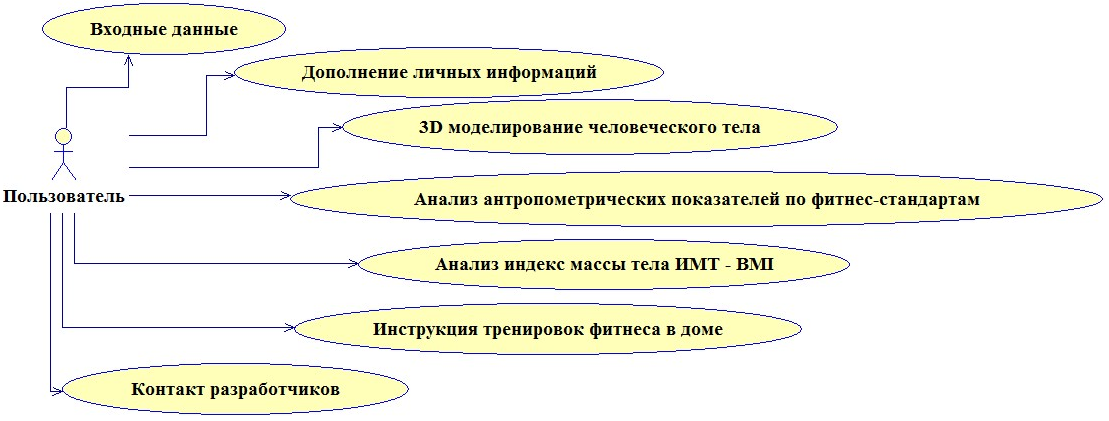
\includegraphics [scale=0.5] {images/h25.png}
\begin{center}
%\captionsetup{justification=justified, labelsep=period}
\caption{Диаграмма прецедентов - использование системы компьютерного зрения приложения E-Fitness.} \label{img25}
\end{center}
\end{figure}
\begin{figure}[ht!]
\centering
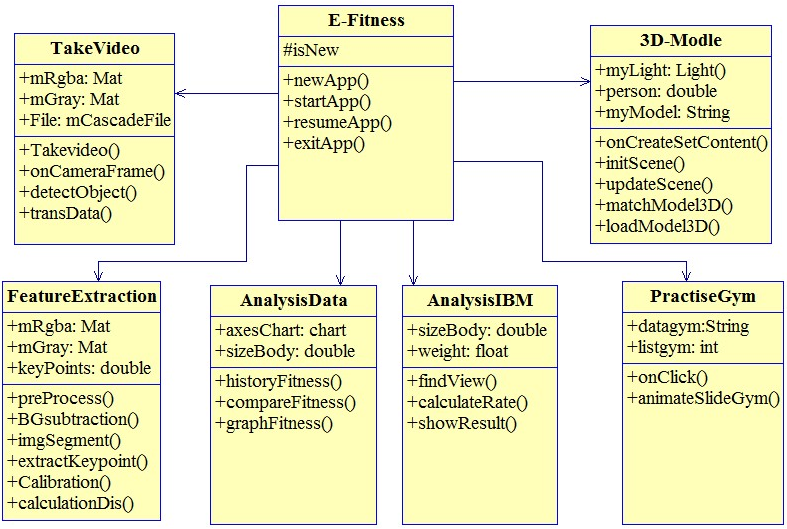
\includegraphics [scale=0.5] {images/h26.png}
\begin{center}
%\captionsetup{justification=justified, labelsep=period}
\caption{Диаграмма классов - система компьютерного зрения в антропометрии приложения E- Fitness.} \label{img26}
\end{center}
\end{figure}
\begin{figure}[ht!]
\centering
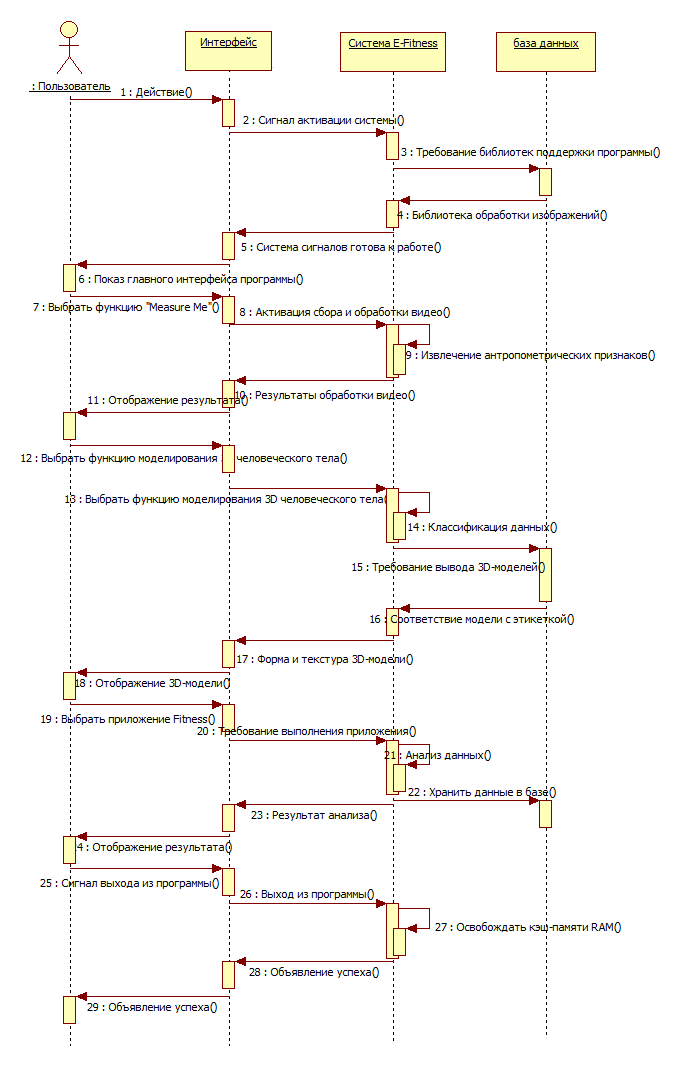
\includegraphics [scale=0.8] {images/h27.png}
\begin{center}
%\captionsetup{justification=justified, labelsep=period}
\caption{Диаграмма последовательности - система компьютерного зрения в антропометрии приложения E- Fitness.} \label{img27}
\end{center}
\end{figure}